\section{The Divine Journey}

A few weeks ago, a young friend was in town. He told me that \textit{Men among the Ruins}, and \textit{Ride the Tiger} were his constant companions, making a large impact on his worldview. Curiously, he then told me that Guenon's \textit{Man and his Becoming} left him cold. Unfortunately for his worldview, Julius Evola wrote this:

\begin{quotex}
Guenon's \textit{Man and his Becoming according to the Vedanta} will draw the attention of the well trained and qualified reader. Of course, it will also become the source of misunderstandings for a certain category of “third rate” critics and intellectuals who oscillate between platitudes and political and spiritual fancies. 

\end{quotex}
I hope my friend will read this article and then proceed on his way to becoming well trained and qualified, but usually sentimentalism supersedes intellect. So the point of a review is to entice readers to return to the original work. There is a reason for it, as Evola explains:

\begin{quotex}
It is only natural that those readers who have followed Guenon's critique [of the modern world] are now curious to learn about the positive counterpart, consisting of the values and doctrines to be opposed to those of the modern world. It is only natural that these readers wish to know what is this `tradition' and the `traditional spirit' so greatly emphasized by Guenon, and which he considers to be the presupposition of any genuine reconstructive work. 

\end{quotex}
Hence, despite Guenon's densely written prose, it is worth the effort to unpack this text. Never forget that Guenon is the master and Evola builds on that foundation, elaborating on his own specific interests. Nevertheless, it should be assumed that Guenon accepts this work, unless he explicitly offers an objection.

\begin{wrapfigure}{rt}{0.35\textwidth}
 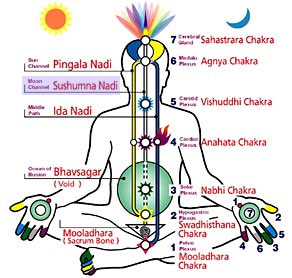
\includegraphics[scale=.5]{a20120823TheDivineJourney-img001.jpg} 
\end{wrapfigure}

Since we have recently been alluding to states of being, the path of the initiate, and postmortem states, we will start near the end with \emph{Chapter XXI: The Divine Journey of the Being on the Path of Liberation}. The final stages of this path assume that a man has reached a certain stage in development symbolized by the coronal artery (\emph{sushumna}) at the crown of the head and connected by a ray to the spiritual Sun. For casual readers, we point out here that any astronomical or elemental symbolism is not to be understood in the material sense.

The being must then follow the way marked by the path of this ray and retracing it back to its source, which is also identical with its destination. We can point out here, in passing, that this is also the esoteric meaning of the stories of Genesis and Exodus, which is repeated in Tradition: it represents the journey from the source to the fall, then to exile in the West and finally the return back to the source. Guenon reminds us that religious conceptions are capable of a transposition to a higher and deeper meaning, something we should always look for instead of rejecting exoteric teachings out of hand (or even accepting their basest interpretation).

This chapter does not deal with the \emph{jivan-mukti}, that is, the being who achieves Deliverance in the human state, but rather with two types of beings:

\begin{enumerate}
\item Beings who obtain Deliverance on leaving the human state 
\item Beings who pass into other states of individual manifestation 
\end{enumerate}
There are, therefore, two corresponding paths:

\begin{enumerate}
\item Path of the Gods (\emph{devayana}) 
\item Path of the Ancestors (\emph{pitriyana}) 
\end{enumerate}
Note that these two paths do not exhaust all the options for postmortem existence. Keep in mind, too, that these paths concern the subtle states of the being, which are still formal and individual, although the corporeal state is no longer part of the being.

Although there are some differences in the order or names of the stages, it may be helpful to compare this to the diagram in Spiritual Beings.

\paragraph{Path of the Ancestors}
Some will recognize this from the descriptions of the way of the ancestors in our series on the Ancient City. Its symbols are: Smoke, night, waning moon, the sun descending to the south. This path is restricted to the Sphere of the Moon\footnote{\url{https://en.wikipedia.org/wiki/Sublunary_sphere}}. Thus, the being is not set free from form or individuality.

The \emph{Sphere of the Moon} represents Cosmic Memory, or the Akashic Record. This is because it is inhabited by the beings of the preceding cycle, who then generate the current cycle. As forms complete the full course of their development, they are dissolved, becoming the germs of undeveloped forms. The end of one state is always the beginning of another.

Thus the being ends one state of existence and begins a new one as an individual in a world of form. Since a being does not occupy the same state twice, the new form does not exist in this world at a later date, as a crude understanding of reincarnation would have it. Nevertheless, it will be in a state of existence, perhaps similar to this one, depending on the possibilities attained in the previous state of existence. This idea is more fully developed in the \emph{Symbolism of the Cross}.

The Lunar Sphere separates the higher, non-individual, states from the lower. This is what separates the two paths. Guenon points to the Litany of the Virgin\footnote{\url{https://www.nashvilledominican.org/prayer/litanies/litany-of-the-blessed-virgin-mary/}} as representing this division, where we read,

\begin{quotex}
Who is she that comes forth as the morning rising, fair as the moon, bright as the sun, terrible as an army set in battle array? \flright{\textsc{Song of Solomon 6:10 }}

\end{quotex}
\paragraph{Path of the Gods}
This path represents those who tend toward Union never to return to manifested existence. Its symbols are: Fire, light, daytime, waxing moon, the sun ascending to the north.

In Vedic symbolism, after leaving the Earth or the world of gross manifestation, i.e., at death, the being is led to the Realm of light, or Fire, ruled by Agni. Then the being is led through the different stages of the \emph{devatas}. In Western symbolism, these stages are said to be ruled by angels. Note, too, that the principle of each stage is personified by a supernatural being. This is not at all insignificant.

Guenon points out that other traditions describe this path and he specifically names the Egyptian Book of the Dead, the Tibetan Bardo Thodol and the Alexandrian Gnostic text Pistis Sophia. He suggests a concordance be written between these texts. 80 years later, this has not yet been done by anyone. We would add to this concordance Ibn Arabi's Meccan Revelations and Dante's Divine Comedy.

As he progresses, the being effectively identifies with the center of the Personality, losing all individual concerns. The effective realization of each state is obtained through identification with the principles of the state. Theoretical knowledge is only a preparation. Transition from one stage to the next is possible only after effective knowledge of the stage. As formless, the being may pass to a Deva or angelic state.

The penultimate stage is the principle of Being, represented by Ishwara. At this point there is no longer any subtle state and the being is in an unmanifested state. The center of the being is identified with the center of all the worlds; this is the same as the fundamental analogy between the macrocosm and the microcosm.  This would persist until the end of the cycle. In Western terms, this is equivalent to Heaven.

\emph{Final Deliverance} is beyond Being, Infinity\footnote{\url{https://www.gornahoor.net/?p=3261}}, comprising Being and non-Being. That is why Guenon's Deliverance is usually called non-dual awareness. The being is liberated from the conditions of individual human existence and well as all other limiting conditions.

\paragraph{Theoretical Preparation}
Guenon provides us with the theoretical preparation for the path; to become gnosis, a man must realize it fully in his heart. Being and Knowing are one. It helps to think about or meditate on these ideas constantly until your entire worldview is permeated with them. Along with that, there is knowing one's true Self, or Atman. This is beyond the individual and is never manifested as such. A question to ponder is:

\textit{What is constant and unchanging in every act of consciousness?}

\flrightit{Posted on 2012-08-23 by Cologero }

\begin{center}* * *\end{center}

\begin{footnotesize}\begin{sffamily}



\texttt{Sparrow on 2015-03-14 at 02:48 said: }

I've been reading a bit about Guenon's view of what happens after death, and while it's logically consistent, I can't really see any reason it's true and the common understanding of reincarnation is false. Almost all ancient teachings that I can recall (Bhagavad Gita, Myth of Er, Bardo Thodol, etc.) don't even come close to suggest a being passes into another state of existence on another plane, never to return to this one. It seems that the opposite case is near universal. While I would be willing to accept that by the fifth century B.C., the ancient teachings had already devolved into reincarnation, Guenon explicitly states this is not the case and that the ancients held the view of transmigration how he describes it.


\end{sffamily}\end{footnotesize}
